% ------------------------------------------------------------------------- %%
\chapter{Conceitos}
\label{cap:conceitos}


\section{Definição do Problema}


Os dados da produção de cimento são anotados temporalmente, então podemos escolher
tratá-los como uma série temporal, i.e. usaremos a ordem temporal como uma informação
relevante na tarefa de aprendizado.
A tarefa de regressão se torna então prever as próximas anotações desses
dados num horizonte de tempo futuro finito.
Na tarefa de aprendizado será usada a série temporal alvo $Y$, dos índices
$RC_{28}$ de resistência compressiva, $Y = \{y_t , t \in \mathbb{Z}^+ \}$.
Também serão usadas séries temporais de
\textbf{covariados}, i.e. variáveis também anotadas temporalmente de composições
químicas de reagentes presentes na produção de cimento, $\textbf{X}$. $\textbf{X} = \{ \textbf{x}_t  \, , t
\in \mathbb{Z}^+  \}$, onde cada $\textbf{x}_t \in \mathbb{R}^K$.

Para k séries temporais de covariados i.e. parâmetros de
entrada. Para simplificar a notação, o índice $t$ será por vezes omitido.

O problema é de Aprendizado Supervisionado(Tópico explicado na
Sessão~\ref{sec:aprenauto}). Usaremos valores passados dos covariados a da
própria série alvo para a predição de novas anotações $y$. A literatura de predição de séries
temporais chama esse tipo de problema onde são usadas valores passadas de uma série
para a predição do futuro da mesma de \textbf{auto-regressão}, para um resumo
das diversas tarefas de aprendizado relacionadas a séries temporais, ver \cite{gluonts}.


Seja um série temporal alvo, $Y$, e diversas séries temporais de variáveis
 $x_k$ com valores nos instantes de tempo no intervalo $[1,T]$. Seja $T$ o último dia em que se possui dados de todas essas
séries. Desejamos modelar a distribuição de probabilidade das próximas anotações
de $y$ até uma nova data $F + T$, $F \in \mathbb{N}$, condicionadas por uma janela de
observações das diversas variáveis  $x_k$ e do alvo $y$ no passado
\citep{deepfactors}. Nota-se que se supõe que possuímos entradas das
variáveis $x_i$ também no período de predição, i.e. no intervalo $[T,F]$.

\[ p(y_{T:F} | y_{1:T},\textbf{x}_{{1}:F}) \]

A distribuição será buscada por meio de aprendizado supervisionado, onde os
modelos serão alimentados com diversos pares de entradas,
$(y_t,\textbf{x}_{t:t+W})$, onde $\textbf{x}$ é um vetor que contém os valores de
cada variável independente $x_i$, no instante de tempo $t$. Cada tupla de
entrada contém $W$ entradas do vetor de entrada. O parâmetro $W$, o
tamanho da janela de tempo consumida para gerar cada saída, é escolhido antes do
treino e pode ser alterado na busca de uma melhor acurácia de predição.



\section{Estatística Frequentista e Estatística Bayesiana}
 
Como nesse trabalho serão usados métodos de inferência Bayesiana aplicados a Aprendizado Automático,
cabe então uma breve elaboração das diferenças entre as duas principais
vertentes da estatística \citep{dlbook}. 

Digamos que exista um evento aleatório que tenha um resultado com probabilidade
$p$ de acontecer. A visão frequentista de probabilidades diz que, se pudéssemos
repetir infinitas vezes esse evento, a proporção de vezes que esse resultado irá
acontecer se aproximará arbitrariamente de $p$. E então entenderíamos a
probabilidade $p$ meramente como uma proporção de resultados positivos em uma
certa amostra de experimentos. Mas e se o evento não pudesse ser repetido?
Quando físicos criam modelos para explicar o nascimento do universo, é
impossível pensar em incerteza como repetições de fenômenos cosmológicos como esse. Nesse segundo caso, resultados são derivados de \textbf{graus de certeza}, onde a chance de um evento acontecer é estimada pela aplicação de conhecimentos prévios em vista de algo que foi observado posteriormente. A primeira maneira de se entender estatística é chamada de Frequentista e a segunda de Bayesiana. \\

E no campo de Aprendizado Automático, as duas maneiras de se gerar predições são estimadores
frequentistas (Seção~\ref{sec:est}) e inferência Bayesiana (seção~\ref{sec:bayesinf}).



\section{Aprendizado Automático}
\label{sec:aprenauto}
O campo de Aprendizado Automático (Machine Learning - Aprendizado Automático) é um ramo da Ciência
da Computação que utiliza métodos estatísticos para criar sistemas que possam
aprender a realizar uma determinada tarefa através de dados. Um problema de Aprendizado Automático possui
as seguintes partes \citep{dlbook}: \\

\begin{itemize}

  
\item A tarefa $T$, no caso dos dados da produção de cimento, um problema de regressão.
  Onde desejamos estimar valores numéricos a partir de uma matriz de dados $X$ e
  suas anotações numéricas $Y$. 
  
\item Uma métrica de performance $P$, que define a distância entre as predições
  do modelo e os dados de treinamento. A teoria por trás desses métricas será explicada na seção~\ref{sec:metricas}.

\item A experiência $E$, que define qual tipo de informação o modelo poderá usar
  durante o treinamento. Explicaremos esse conceito na seção~\ref{sec:exp} 
  
\end{itemize}

\subsection{A Experiência}
\label{sec:exp}
Algoritmos de Aprendizado Automático podem ser divididos nas categorias de
aprendizado supervisionado, não supervisionado e aprendizado por reforço
\citep{dlbook}. Técnicas dos dois primeiros tipos serão usadas para os dados de
produção de cimento.


\subsubsection{Aprendizado Supervisionado}
\label{sec:apren} 
Aprendizado Supervisionado consiste, do ponto de vista estatístico, no
aprendizado de uma distribuição de probabilidade do tipo $p(y | x)$. Uma
regressão linear pode ser entendida como a distribuição do alvo $y$, $p(y | x) = \theta^Tx + \epsilon =
\mathcal{N}(\theta^Tx,\sigma) $, $\epsilon \sim \mathcal{N}(0,\sigma)$. Esse ponto será melhor
explorado na Sessão~\ref{sec:est}. \\ 

Dados vetores de entrada $x$ associados a uma anotação $y$, a tarefa consiste na busca de uma
função dentro de uma família de funções que melhor generalize a relação entre
$x$ e $y$. De modo que os modelos possam gerar anotações inéditas $y'$ para
dados $x'$ nunca antes vistos. 


\subsubsection{Aprendizado Não Supervisionado}

Para o caso de Aprendizado Não Supervisionado, mantendo a estrutura do exemplo
anterior, desejaríamos então modelar uma distribuição do tipo $p(x)$, onde temos
também diversos exemplos de vetores aleatórios $x$ e estamos estudando alguma
propriedade importante dessa distribuição.
Esse tipo de problema é mais comum em tarefas de Visão Computacional e NLP.



\subsection{A Performance}
\label{sec:metricas}

A performance dos modelos de aprendizagem automática é a quantificação da
qualidade das predições frente a verdade desconhecida do fenômeno modelado.
Claramente um modelo parametrizado possuirá algum erro de predição \cite{dlbook}, e é esse
erro que iremos diminuir com o aprendizado. Os estimadores serão a ferramenta
usada para guiar o treinamento em uma direção que reduza ao máximo o viés das predições.

\subsubsection{O fenômeno do perde-e-ganha entre viés e variância}

Seja um modelo treinado de aprendizagem automática representado por uma função
$\hat{f}$, que recebe como domínio valores de $x \in \mathbb{R}$, os dados de
entrada. Iremos estudar como se comporta o valor esperado do erro quadrático do
modelo, i.e. $\mathbb{E}[(y - \hat{f}(x))^2]$, onde $y$ é o valor real porém
desconhecido da saída. Estudando esse valor, podemos decompô-lo em
3 partes \citep{mlprob}:

\[
  \mathbb{E}[(y - \hat{f}(x))^2] = \text{Viés}[\hat{f}(x)]^2 +
  \text{Var}[\hat{f}(x)] + \sigma 
\]

O erro quadrático médio de um modelo de aprendizado
é sempre composto por esses 3 termos. O viés nos informa o valor esperado do
erro das predições, i.e. um modelo sem viés tem a sua média de predições
consistente com o valor real. Porém, por mais que um modelo sem viés seja
altamente desejável, esse termo de erro deve ser negociado em frente a variância
das predições, o segundo termo. Por mais que a média das predições de um modelo
se aproximem do valor real, isso de nada adianta se, por diversos ruídos na
modelagem, o modelo apresentar uma alta sensibilidade a pequenas alterações em
parâmetros ou dados, i.e. uma alta variância nas predições.

O último termo do erro denotado por $\sigma$ é a parte aleatória do erro
impossível de ser reduzida devido a impossibilidade de modelagem de toda a
distribuição geradora dos dados.

\subsubsection{Estimadores}
\label{sec:est}

A aprendizagem estatística busca a diminuição de \textit{risco empírico} das predições feitas por
um modelo \citep{mlprob}. O risco empírico é dado pelo somatório de uma função
de custo por todo o conjunto de dados:

\[
  \mathcal{L} = \frac{1}{T}\sum_{t=0}^{i=T}L(y_t,\hat{y_t}) 
\]

Um método possível da diminuição de risco é o de guiar o aprendizado pela
maximização da verossimilhança do modelo. Esse valor é a probabilidade de termos
observado os dados alvo condicionada pelos parâmetros do modelo e as entradas
(que iremos representar pelo vetor $\theta$). Uma iteração de
treino então consistira do produtório de todas as verossimilhanças para cada par
de entradas. Na definição do nosso problema, temos que o custo total do modelo
$\mathcal{L}$ é dado pela seguinte equação \citep{dlbook}, considerando que o
modelo recebe $W$ entradas temporais para o calculo da verossimilhança de uma saída:

\[
\mathcal{L} = \prod_{t=0}^{i=T} p(y_t | \textbf{x}_{t}, \theta) 
\]

É comum, porém, por motivos de estabilidade numérica \citep{dlbook}, substituir
o produtório de probabilidades pelo somatório do logarítimo das probabilidades: 

\[
  \mathcal{L} = \sum_{t=0}^{i=T} \log{p(y_t | \textbf{x}_{t},\theta)}
\]

Em uma análise bayesiana, também buscaríamos maximizar a verossimilhança dos
dados condicionados aos parâmetros do modelo. Mas como exige a formalização
bayesiana, iriamos considerar uma distribuição a priori dos parâmetros do
modelo, i.e. $p(\theta)$:


\[
  \mathcal{L} = \prod_{t=0}^{i=T}p(y_t|\textbf{x}_{t},\theta)p(\theta) 
\]


Para modelos com baixa dimensionalidade e muitos dados, a estimativa bayesiana
coincide com a frequentista, convergindo para a \textbf{estimação de máxima
verossimilhança} \citep{mlprob}. Isso se deve ao fato que a distribuição de
probabilidade a priori progressivamente se torna menos importante no calculo da
probabilidade posterior com muitos dados. Por isso se diz que a Inferência
Bayesiana é um estimador consistente \citep{mlprob}, i.e. ele converge para uma
hipótese arbitrariamente próxima da verdade.


Na seção~\ref{sec:reglog} iremos dar um exemplo dessa cálculo de verossimilhança
assumindo que o erro do modelo é distribuído normalmente.

\subsubsection{A Distribuicão Normal}
\label{sec:reglog}

Uma variável aleatória Y distribuída normalmente possui uma função densidade de
probabilidade da seguinte forma \citep{mlprob}:

\begin{equation}
  \label{eq:ver}
p(y| \mu,\sigma^2) = \frac{1}{\sqrt{2\pi\sigma^2}}\exp{-\frac{(y - \mu)^2}{2\sigma^2}}
\end{equation}

Esse valor também é chamado de verossimilhança (a probabilidade de termos
observado um valor de Y, dado que essa variável é distribuída normalmente, com média $\mu$ e variância $\sigma^2$), e
normalmente trabalha-se com o logaritmo desse valor, para podermos trocar um
produtório por somatório para agregar os erros gaussianos de um conjunto de dados
i.i.d.. Nesse caso, temos pares de predição e valor real, que assumirá o papel
da média $\mu$. A verossimilhança total de um conjunto de diversos pares
$(\hat{y},y)$ é dado por: 

\begin{equation}
\label{eq:logver1}
  \mathcal{L}= -m \log \sigma - \frac{m}{2} \log (2 \pi) - \sum^m_{i=1}
  \frac{\abs{\hat{y_i}-y_i}^2}{2 \sigma^2}
\end{equation}

Um estimador sem viés da Equação~\ref{eq:logver1}, chamado de Erro Quadrático
Médio, pode ser escrito apenas como \citep{mlprob}:

\begin{equation}
  \label{eq:logver2}
  \mathcal{L}=  \sum^m_{i=1} (\hat{y_i}-y_i)^2
\end{equation}


\subsubsection{Função de Custo}

A Função de Custo é uma função usada para guiar os algoritmos de otimização na
direção de parâmetros que melhorem a performance do modelo \citep{dlbook}.
Essa função para alguns modelos pode representar a verossimilhança dos dados,
mas isso não é necessário no geral.

Nessa sessão iremos definir a função de custo usada em todos os modelos de regressão usados. \\

\subsubsection{Erro Quadrático Médio}
\label{sec:MSE}

O Erro Quadrático Médio é um estimador não enviesado da Equação~\ref{eq:ver}
\citep{dlbook} para o cálculo da verossimilhança de um modelo Gaussiano. Ele é calculado em relação a duas variáveis contínuas
$(\hat{y},y)$, definido da seguinte forma:

\[MSE = \sum^n_{i=1}\frac{(\hat{y_i} - y_i)^2}{n}\]

Essa métrica é uma medida absoluta. E quanto maior esse valor pior o desempenho
do modelo, i.e. mais distante suas predições estão da média real. \\

\subsubsection{Divergência KL}

A divergência KL, ou Kullback-Leibler, é uma medida de diferença entre duas distribuições de probabilidade (também chamada de Entropia Relativa). \\
Essa medida pode ser definida pelo valor esperado da diferença logarítmica da probabilidade dos dados serem observados em uma distribuição ou na outra \citep{dlbook}. \\
Sejam duas distribuições de probabilidade $p$ e $q$, bem como uma matriz de dados $X$: \\

\[D_{KL}(p || q) = \mathop{\mathbb{E}}[\log p(x) - \log q(x)]​\]

Ou em uma forma mais usual: \\

\[D_{KL}(p||q) = \sum_{i=1}^{N}p(x_{i}) \log \frac{p(x_{i})}{q(x_{i})}​\]



\subsection{Métrica de Acurácia}

Diferentemente da função de custo, a métrica de acurácia não é usada para guiar a otimização do modelo,
mas para testar as predições frente a realidade e avaliar sua qualidade. \\

\subsubsection{R-quadrado}
Como teste da acurácia dos modelos foi usada a métrica R-quadrado ($R^2$) \citep{cohen}. Sejam $\hat{y}$ e $y$ nossa previsão dada pelo modelo e o seu valor real, a acurácia do modelo é dada por:\\

\begin{align}
&R^2 = 1 - \frac{SS_{res}}{SS_{tot}} &\\
&SS_{tot} = \sum^n_{i=1} (y_i- \bar{y_i})^2 &\\
&SS_{res} = \sum^n_{i=1} (y_i - \hat{y})^2 &\\
&\bar{y} = \frac{1}{n} \sum^n_{i=1} y &
\end{align}

% \justify
$SS_{res}$ mensura a quantidade de variância \textit{residual}, a
variância entre os dados reais e as predições do modelo, i.e. a variância não
explicada pelo modelo. $SS_{tot}$ cumpre o papel da variância \textit{total}. A métrica $R^2$
então nos mostra quanto da variância dos dados é explicada pelo modelo. \\

Para essa métrica, o modelo pode ter um desempenho arbitrariamente ruim, com esse valor
podendo se tornar arbitrariamente negativo. Porém, seu valor máximo é 1,
indicando um modelo ideal.\\


\subsubsection{Custo quantílico}
\label{sec:quant}
O custo quantílico \citep{deepar} é usado na avaliação de performance de
predições temporais. \\

Para uma predição com desvio-padrão $\sigma$, um quantil $q$ representa o
valor que cobre $\rho\%$ da distribuição de probabilidade dessa predição.

Por exemplo, usando o quantil $\rho=0.9=90\%$, podemos calcular quantos
desvios-padrões cobrem $90\%$ dos valores presentes na distribuição.
Assumindo distribuição normal das predições, com média $y^*$, para $\rho=0.9$, uma tabela z nos mostra que devemos usar $1.29$ desvios-padrões:

\[
  y^*(\rho = 0.9) = y^* + 1.29\sigma
\]

Logo, $y^*(0.9)$ cobre $90\%$ dos possíveis valores de predição feitos pelo
modelo, levando em consideração o desvio-padrão.

Dado um quantil $\rho \in (0,1)$ um valor real $y_{t}$ e um quantil de previsão 
$y^{*}_{t}(\rho)$, define-se o custo quantílico por: \\

\begin{equation}
  \mathcal{QL}_{\rho}(y_{t},y^{*}_{t}(\rho)) =
\begin{cases*}
  2 \rho(y_{t} - y^{*}_{t}(\rho)) & se $ y_{t} - y^{*}_{t}(\rho) > 0$ \\
  2 (1 - \rho)(y^{*}_{t}(\rho) - y_{t}) & se $y_{t} - y^{*}_{t}(\rho) \leq 0$
\end{cases*}
\end{equation}


Esse valor é somado em todas as séries temporais $i$ no horizonte de predição
representado pelos valores de $t$ e normalizado usando os valores da série temporal.


\[
   p(\rho)QL = \frac{\sum_{i,t}\mathcal{QL}_{\rho}(y_{t},y^{*}_{t}(\rho))}{\sum_{i,t}\abs{y_{i,t}}}
\]


Esse valor é bastante informativo quando as saídas dos modelos são distribuições
de probabilidades. Esse valor nos informa o risco ponderado de um certo quantil
da predição.

Se usarmos o quantil $\rho=0.5=50\%$, p50QL,
esse valor se torna a porcentagem absoluta média de erro (MAPE). Para
$\rho=0.9=90\%$, p90QL, será
calculado o erro máximo esperado por $90\%$ das predições.



%% ------------------------------------------------------------------------- %%


\section{Abordagem Não-Temporal} 


\subsection{Redes Neurais}

\label{sec:nn}
Redes neurais são aproximadores universais de funções \citep{nnuni}. Dado um problema
de classificação onde se deseja aprender uma função da forma $y = f^*(x)$, uma
Rede Neural define um mapeamento $y = f(x ; \theta)$, onde $\theta$ é o vetor de
parâmetros que serão aprendidos com o fim de minimizar a diferença entre a
distribuição empírica e essa distribuição gerada pelo modelo. Essa diferença pode
ser minimizada pelo método da verossimilhança, assim como elaborado na sessão~\ref{sec:reglog}.\\

O modelo neural é uma composição de funções que unem uma transformação linear e
a aplicação de uma função não-linear $\sigma$: \\

\[ f(x)=  \sigma(W*x + b) \]

Importante ressaltar que $W$ é uma matriz, assim como $x$ e $b$ são vetores. \\

A computação da saída de uma rede neural então pode ser escrita como:

\[   y = f_n \circ f_{n-1} \circ f_{n-2} \dots f_1(x)  \]

Para uma rede neural de $n$ \textbf{camadas}, onde cada camada será uma função
$f_i$ cujos parâmetros são $W_i$ e $b_i$. Portanto, para a i-ésima camada da rede
sua saída será da forma: 

\[ f_i (x)=  a_i = \sigma(W_i*a_{i-1} + b_i) \]

Onde $a_{i-1}$ é a saída da camada anterior, também chamada de
\textbf{ativação}. A saída dessa camada é então a sua ativação $a_i$. \\ 

Vale notar que uma saída $y$ calculada por uma rede neural depende unicamente dos
seus parâmetros e da entrada $x$. Isso não será verdade para os modelos
\textbf{sequenciais} que também serão usados nesse trabalho, onde o estado
interno de computação desses modelos é usado como entrada para uma próxima
iteração \citep{dlbook}. \\

Na Figura~\ref{fig:nn} mostramos como seria uma rede que usa os índices RC3 e RC7 para
modelar como saída o índice RC28. \\  

\begin{figure}
  \centering
  \def\layersep{2.5cm}

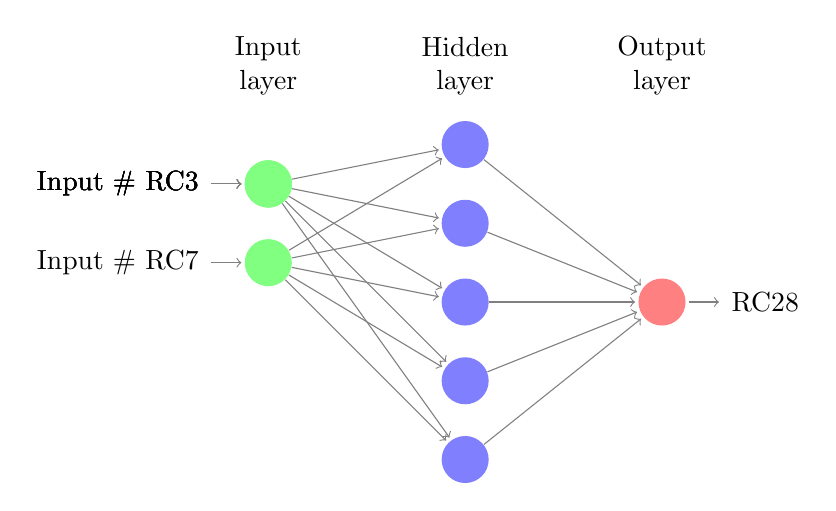
\begin{tikzpicture}[shorten >=1pt,->,draw=black!50, node distance=\layersep]
    \tikzstyle{every pin edge}=[<-,shorten <=1pt]
    \tikzstyle{neuron}=[circle,fill=black!25,minimum size=17pt,inner sep=0pt]
    \tikzstyle{input neuron}=[neuron, fill=green!50];
    \tikzstyle{output neuron}=[neuron, fill=red!50];
    \tikzstyle{hidden neuron}=[neuron, fill=blue!50];
    \tikzstyle{annot} = [text width=4em, text centered]

    % Draw the input layer nodes
    \foreach \name / \y in {1,...,4}
    % This is the same as writing \foreach \name / \y in {1/1,2/2,3/3,4/4}
    \node[input neuron, pin=left:Input \# RC3] (I-1) at (0,-1) {};
    \node[input neuron, pin=left:Input \# RC7] (I-2) at (0,-2) {};

    % Draw the hidden layer nodes
    \foreach \name / \y in {1,...,5}
        \path[yshift=0.5cm]
            node[hidden neuron] (H-\name) at (\layersep,-\y cm) {};

    % Draw the output layer node
    \node[output neuron,pin={[pin edge={->}]right:RC28}, right of=H-3] (O) {};

    % Connect every node in the input layer with every node in the
    % hidden layer.
    \foreach \source in {1,...,2}
        \foreach \dest in {1,...,5}
            \path (I-\source) edge (H-\dest);

    % Connect every node in the hidden layer with the output layer
    \foreach \source in {1,...,5}
        \path (H-\source) edge (O);

    % Annotate the layers
    \node[annot,above of=H-1, node distance=1cm] (hl) {Hidden layer};
    \node[annot,left of=hl] {Input layer};
    \node[annot,right of=hl] {Output layer};
\end{tikzpicture}
  \caption{Um exemplo de Rede Neural no contexto dos dados de produção de cimento}
  \label{fig:nn}
\end{figure}


\bigskip

\subsubsection{Regularização L2}

Em \cite{dlbook}, os autores definem regularização como \say{qualquer
  modificação em um algoritmo de aprendizado que diminua o erro de generalização
mas não o seu erro de treinamento}. A ideia é se colocar informação objetivo de 
otimização que diminua a complexidade do modelo encontrado, fazendo assim
que o modelo tenha menos capacidade de aprender a modelar o ruído inerente
aos dados de treinamento, i.e. a parte dos dados que é atribuída a erros
impossíveis de serem modelados.

A regularização L2 consiste em adicionar a norma quadrada de todos os parâmetros
do modelo ao objetivo de otimização. Dessa maneira o algoritmo é levado a
encontrar valores menores para os parâmetros, visto que a otimização é
direcionada a achar o menor valor possível do objetivo.



\section{Modelos Sequenciais}

Modelos sequenciais consomem sequências de dados e também podem ser usados pra
criar predições sequenciais \citep{dlbook}. A área de NLP viu muitos novos
resultados com o uso esses tipos de modelos para geração e classificação de textos, que são dados com
natureza inerentemente sequencial. Para o caso desse trabalho, séries temporais também podem
aproveitar da capacidade desses modelos de lerem multiplas entradas ao mesmo
tempo. Modelos sequenciais são bastante comuns para processamento de texto e
áudio e outras famílias de dados cuja natureza é eminentemente uma sucessão de
eventos no tempo. Dados de processos industriais comumente se encaixam nessa
categoria, inclusive produção de cimento, logo, passíveis de serem usados
juntamente com esses modelos.



\subsection{Janela Móvel com Filtragem Exponencial}
\label{ses:ewma}

A abordagem usada em \cite{grecialin} consiste em calcular regressões lineares em
uma janela móvel de dados, simulando limitações reais do chão de fábrica. O
objetivo da regressão é sempre o índice RC28 de um determinado lote de cimento,
do qual possuímos análises químicas e resultados de outros ensaios usados como
variáveis. Essa abordagem irá utilizar a ordem temporal desses dados para
modelagem e predições. Diferentes conjuntos de variáveis serão usados dependendo
da sua disponilidade considerando a ordem e dia que essas ficam disponíveis na
operação normal da fábrica.

Para um dia $t$ possuímos $RC28_t$ e $\textbf{x}_t$, respectivamente o objetivo
da regressão e o vetor de entradas. A Tabela~\ref{tb:vars} determina quais entradas estão presentes em $\textbf{x}_{t}$ para cada modelo usado.
Seja o dia $T$ onde começa a aplicação do modelo. Acaba de ficar pronto o ensaio
de RC28 do lote expedido 29 dias no passado, i.e. $RC28_{T-29}$.  O dataset móvel está no
intervalo $[T-29-t_d,T-29]$ i.e. os pares
$\{(\textbf{x}_{T-29-t_d},RC28_{T-29-t_d}), (\textbf{x}_{T-28-t_d},RC28_{T-28-t_d})
\dots (\textbf{x}_{T-29},RC28_{T-29})\}$, $t_d$ um hiper-parâmetro.

Usa-se esse dataset para calcular pesos de 3 regressões diferentes para a predição de RC28.


% copiar output do pandas aqui
% esta no notebook papergrecia
\begin{table}[]
  \centering 
  \begin{tabular}{llllllllllllll}
    \toprule
    reglin\_1 &  AGP &  AL2O3 &  SIO2 &  MGO &  IP &  FP &  SBL &  PF &  P2O5 &  FE2O3 &  RC1 &      &      \\
    reglin\_3 &  AGP &  AL2O3 &  SIO2 &  MGO &  IP &  FP &  SBL &  PF &  P2O5 &  FE2O3 &  RC1 &  RC3 &      \\
    reglin\_7 &  AGP &  AL2O3 &  SIO2 &  MGO &  IP &  FP &  SBL &  PF &  P2O5 &  FE2O3 &  RC1 &  RC3 &  RC7 \\
    \bottomrule
  \end{tabular}
  \caption{O conjunto de variáveis usado para cada um dos modelos, de maneira análoga ao apresentado no trabalho \cite{grecialin}}
  \label{tab:modelslin}
\end{table}


No dia $T$ acabaram de ficar prontos os ensaios RC1, RC3 e RC7 respectivamente
dos lotes expedidos nos dias $T-2$,$T-4$ e $T-8$. Os modelos descritos na 
Tabela~\ref{tab:modelslin} e treinados com o dataset do período 
$[T-29-t_d,T-29]$ são aplicados para prever o RC28 de acordo com a
disponibilidade dos ensaios nessas 3 datas. reglin\_1 é aplicado em $T-1$
para prever $RC28_{T-1}$,
reglin\_3 em $T-4$ para prever $RC28_{T-4}$ e reglin\_7 em $T-8$ para prever
$RC28_{T-8}$.

Continuamos aplicando os modelos por $t_f$ dias,
no dia $T+1$, por exemplo, iremos poder aplicar reglin\_1,reglin\_3 e
reglin\_7 respectivamente nos dias $T-1$,$T-3$ e $T-7$ e gerar novas predições
para RC28 nessas datas.  

A Tabela~\ref{tab:ranges} mostra para cada modelo os intervalos de
datas usadas para treinamento e predição, usando $t_d$ e $t_f$ como parametros
que determinam o tamanho do dataset móvel e do horizonte de predição, respectivamente.


\begin{table}[]
  \centering 
  \begin{tabular}{lll}
    Modelo    & Intervalo de Treinamento & Intervalo de Predição \\
    reglin\_1 & $[T-29-t_d,T-29]$        & $[T-1, T-1+t_f]$      \\
    reglin\_3 &  $[T-29-t_d,T-29]$       &  $[T-4, T-4+t_f]$      \\
    reglin\_7 &   $[T-29-t_d,T-29]$      &   $[T-8, T-8+t_f]$       
  \end{tabular}
  \caption{Intervalos de tempo usados como dados de treinamento e predição dos modelos.}
  \label{tab:ranges}
\end{table}


Após $t_f$ dias um novo dataset é escolhido para recalcular os parâmetros das regressões e repete-se o processo com $T' = T + t_f$.

Um quarto modelo é criado corrigindo as predições de reglin\_1 com as de
reglin\_7, esse modelo será nomeado reglin\_ew. Primeiramente calcula-se a
diferença entre as predições de $reglin\_7$ e as medidas reais de RC28 para o período
$[T-29,T-29 + t_f]$, visto que usamos os modelos por $t_f$ dias, novas
anotações de RC28 se tornaram disponíveis nesse período. 


\[
  \mathit{diff}_i = reglin\_7_i - RC28_i
\]

É aplicada então uma média móvel exponencial no vetor diff, com parâmetro
$\alpha$, cujo resultado é o vetor filtrado diff\_ew. O algoritmo da média móvel
é mostrado na Equação~\ref{eq:ew}:


  \begin{align}
    \mathit{diff\_ew}_0 &= \mathit{diff}_0 \\
  \mathit{diff\_ew}_t &= (1- \alpha)\mathit{diff}_{t-1} + \alpha \mathit{diff}_t 
  \label{eq:ew}
  \end{align}


O valor das predições de reglin\_1 são então corrigidos usando o vetor filtrado
diff\_ew. Os intervalos usados (emparelhados) são $t \in [T-1,T-1+t_f]$ para
reglin\_1 e $i \in [T-29,T-29+t_f]$ para diff\_ew. $k$ também é um hiper-parâmetro.

\[
reglin\_ew_t = reglin\_1_t + k * \mathit{diff\_ew}_i
\]


Levantando-se os erros quadráticos para os 4 modelos em seus períodos de
teste, escolhem-se os hiper-parâmetros $t_d$, $k$ e $\alpha$. $t_f$ pode ser
escolhido de acordo com a necessidade de controle de qualidade da fábrica. Nos
testes realizados nesse trabalho, usamos $t_f=7$ para efeito de comparação com
os modelos de Aprendizagem Profunda. 

\subsection{Rede Neural Recorrente}
% 
\scalebox{1}{
\begin{tikzpicture}[auto]

% RNN state cell =============================
\node[state] (h) {$\vect{h}$};
\node[op, below=30pt of h] (x) {$\vect{x}$};
\node[op, above=30pt of h] (yhat) {$\hat{\vect{y}}$};



% edges
\path[tedge] (x) edge node[below right= -4pt] {$\vect{U}$}  (h) ;
\path[tedge] (h) edge [out=-400,in=-320,looseness=8, distance=125pt] node[above right] {$\vect{W}$} (h);
\path[tedge] (h) edge node[below right = -4pt] {$\vect{V}$} (yhat);


\end{tikzpicture}
} % scalebox


A família das Redes Neurais Recorrentes (RNN) é composta por modelos especializados
em processar dados sequenciais \citep{dlbook}, da forma $x^{(1)},x^{(2)} ,x^{(3)}\dots ,x^{(T)}$. Uma rede neural recorrente é definida por uma função com
\textbf{recorrência} ou \textbf{recursão}, de modo que no processamento de uma
sequência o estado da rede seja de certo modo propagado temporalmente. A equação
a seguir ilustra uma função com recorrência: \\

\[h^{(t)} = f(h^{(t-1)},x^{(t)};\theta)\]

Nessa equação notamos que na iteração $t$ o valor do vetor $h$ depende de
$h_{t-1}$.RNNs aprendem a usar esse vetores como
\say{resumos} das iterações passadas. Desse modo , o modelo ganha a capacidade
de usar informações passadas da sequência para o cálculo
de uma saída. Essa capacidade porém começa a ser dificultada quando o modelo
realiza muitas iterações temporais. Durante o aprendizado, sequências muito
extensas criam problemas numéricos para o cálculo dos gradientes, esses podendo
tomar valores muito pequenos ou muito grandes, esse fenômeno recebe o nome de
\textbf{gradientes desaparecidos}. Foram propostos outros modelos
que não possuam esse problema, como o modelo LSTM, explicado na sessão~\ref{sec:lstm}. 

%%%
\begin{figure}[H]
\centering
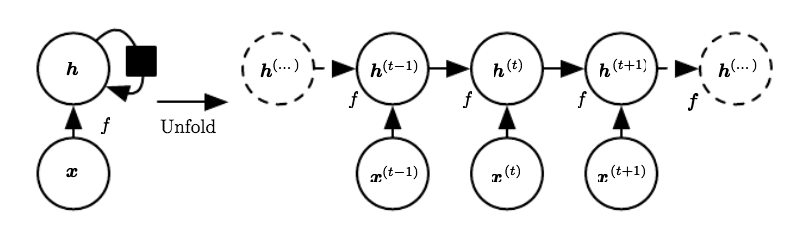
\includegraphics[width=0.9\columnwidth]{rnn.png}
\caption{Grafo de Computação de uma RNN genérica \citep{dlbook}}
\label{fig:rnngraph}
\end{figure}
%%%

Como podemos ver na Figura~\ref{fig:rnngraph}, a entrada $x$, ao lado do estado
interno $h$, são usados para calcular um novo estado. Nota-se que o vetor $h$,
bem como os parâmetros internos da RNN, são divididos entre iterações temporais.
\\

Essa classe de modelos normalmente é usada para modelagem de linguagem. Buscando
estimar uma distribuição de probabilidade $p(w_t | w_{t-1},w_{t-2},w_{t-3} \dots
) $ onde os $w_i$ são palavras subsequentes de um texto. Normalmente um modelo
dessa natureza busca resolver um problema de classificação, onde a próxima palavra
a ser prevista pelo modelo é uma entre todas as possibilidades de um certo
vocabulário. No caso do domínio em questão desejamos resolver um problema de
regressão, onde nosso alvo é um valor numérico. Para treinar um desses modelos,
precisamos usar como entrada exemplos subsequentes de dados, onde cada exemplo
de entrada tem um exemplo pareado de saída. Basicamente redes neurais
recorrentes funcionam recebendo um exemplo de entrada, criando uma representação
interna com o mesmo e então gerando uma saída e comparando essa saída com o
exemplo de saída real, gerando um erro. Finalmente, esse erro é propagado para
alterar seus parâmetros (com o fim de achar um conjunto de parâmetros que gere
boas previsões). \\ 


Como já explicado anteriormente, nossos dados de entrada e saída não estão necessariamente pareados perfeitamente dia a dia. Portanto, foi necessário achar intervalos de tempo nos dados onde existe esse pareamento. Isso reduz drasticamente quais períodos representados nos dados realmente podem ser usados para treinar um desses modelos.


\subsubsection{LSTM}
\label{sec:lstm}

LSTMs \citep{lstm} são um tipo de RNN que por meio de sua arquitetura permitem que sequências
maiores sejam processadas sem que o fluxo dos gradientes propagados pela rede se torne
numericamente problemático (i.e. tendendo a 0 ou a infinito). A
Figura~\ref{fig:lstm} ilustra o fluxo dos sinais em uma LSTM. Observa-se que a
entrada $x_t$ e o antigo estado $h_{t-1}$ são usados para o cálculo de diversos \textit{gates} ou \say{portas}, e
finalmente um novo estado $h_t$ é gerado.\\

\begin{figure}
\centering
\caption{Diagrama da arquitetura de uma LSTM}


\begin{tikzpicture}[
    prod/.style={circle, draw, inner sep=0pt},
    ct/.style={circle, draw, inner sep=5pt, ultra thick, minimum width=10mm},
    ft/.style={circle, draw, minimum width=8mm, inner sep=1pt},
    filter/.style={circle, draw, minimum width=7mm, inner sep=1pt, path picture={\draw[thick, rounded corners] (path picture bounding box.center)--++(65:2mm)--++(0:1mm);
    \draw[thick, rounded corners] (path picture bounding box.center)--++(245:2mm)--++(180:1mm);}},
    mylabel/.style={font=\scriptsize\sffamily},
    >=LaTeX
    ]

\node[ct, label={[mylabel]Cell}] (ct) {$c_t$};
\node[filter, right=of ct] (int1) {};
\node[prod, right=of int1] (x1) {$\times$}; 
\node[right=of x1] (ht) {$h_t$};
\node[prod, left=of ct] (x2) {$\times$}; 
\node[filter, left=of x2] (int2) {};
\node[prod, below=5mm of ct] (x3) {$\times$}; 
\node[ft, below=5mm of x3, label={[mylabel]right:Forget Gate}] (ft) {$f_t$};
\node[ft, above=of x2, label={[mylabel]left:Input Gate}] (it) {$i_t$};
\node[ft, above=of x1, label={[mylabel]left:Output Gate}] (ot) {$o_t$};

\foreach \i/\j in {int2/x2, x2/ct, ct/int1, int1/x1,
            x1/ht, it/x2, ct/it, ct/ot, ot/x1, ft/x3}
    \draw[->] (\i)--(\j);

\draw[->] (ct) to[bend right=45] (ft);

\draw[->] (ct) to[bend right=30] (x3);
\draw[->] (x3) to[bend right=30] (ct);

\node[fit=(int2) (it) (ot) (ft), draw, inner sep=0pt] (fit) {};

\draw[<-] (fit.west|-int2) coordinate (aux)--++(180:7mm) node[left]{$x_t$};
\draw[<-] ([yshift=1mm]aux)--++(135:7mm);
\draw[<-] ([yshift=-1mm]aux)--++(-135:7mm);

\draw[<-] (fit.north-|it) coordinate (aux)--++(90:7mm) node[above]{$x_t$};
\draw[<-] ([xshift=1mm]aux)--++(45:7mm);
\draw[<-] ([xshift=-1mm]aux)--++(135:7mm);

\draw[<-] (fit.north-|ot) coordinate (aux)--++(90:7mm) node[above]{$x_t$};
\draw[<-] ([xshift=1mm]aux)--++(45:7mm);
\draw[<-] ([xshift=-1mm]aux)--++(135:7mm);

\draw[<-] (fit.south-|ft) coordinate (aux)--++(-90:7mm) node[below]{$x_t$};
\draw[<-] ([xshift=1mm]aux)--++(-45:7mm);
\draw[<-] ([xshift=-1mm]aux)--++(-135:7mm);
\end{tikzpicture}


%%% Local Variables:
%%% mode: latex
%%% TeX-master: '../quali'
%%% End:

\label{fig:lstm}
\end{figure}




Uma rede LSTM possui três \say{portas}. Cada porta possui duas matrizes $W,U$ e um
vetor $b$ de parâmetros. Uma iteração da LSTM começa com o cálculo dos sinais
$o_t,i_t,f_t$.\\

\[f_t = \sigma_g(W_fx_t + U_fh_{t-1} + b_f)\]
\[i_t = \sigma_g(W_ix_t + U_ih_{t-1} + b_i)\]
\[o_t = \sigma_g(W_ox_t + U_oh_{t-1} + b_o)\]

O diferencial de uma LSTM é a propagação do sinal $c_t$, a célula de memória.
Esse valor depende de $f_t$ e $i_t$, que influenciam em como o valor da
célula de memória será atualizado na presente iteração. A equação a seguir
mostra como o valor da célula de memória é calculado. Onde $\circ$ é o produto Hadamard, ou apenas multiplicação entrada por entrada de
duas matrizes ou vetores. \\

\[c_t = f_t \circ c_{t-1} + i_t \circ \sigma_c(W_cx_t + U_ch_{t-1} + b_c)\]

Nota-se que $f_t$
define quanto do valor antigo da célula de memória deve participar no cálculo do
seu novo valor. 
Da mesma maneira $i_t$ define quanto da nova entrada deve ser usada no cálculo desse valor.
Em outras palavras, as portas $i_t$ e $f_t$ definem o quanto a LSTM deve,
respectivamente, \say{lembrar} e \say{esquecer}.


O novo estado da LSTM é então calculado por: \\
\[h_t = o_t \circ \sigma_h(c_t)\]




\subsubsection{Rede Encoder-Decoder}
\label{sec:encdec}
Redes Encoder-Decoder são usadas para modelagem de sequência para
sequência, ou seja, para receber dados sequenciais como entrada e gerar
sequências como saída \citep{dlbook}. Esses modelos possuem duas partes, ambas compostas por
RNNs. \\

\begin{figure}[H]
\centering
\begin{tikzpicture}[font=\sffamily]
\node[fill=brown!90!black, text=white, font=\sffamily\small, inner sep=2pt] (a) {\begin{tabular}{@{}r@{}}-0.2\\-0.1\\0.1\\0.4\\-0.3\\1.1\end{tabular}};

\node[fit=(a.north) (a.south), inner sep=1pt, right=1mm of a, minimum width=2cm, label=center:Decoder] (dec) {};
\node[fit=(a.north) (a.south), inner sep=1pt, left=1mm of a, minimum width=2cm, label=center:Encoder] (enc) {};

\begin{scope}[on background layer]
\fill[cyan!30] (dec.north west)--([yshift=5mm]dec.north east)--([yshift=-5mm]dec.south east)--(dec.south west)--cycle;
\fill[cyan!30] (enc.north east)--([yshift=5mm]enc.north west)--([yshift=-5mm]enc.south west)--(enc.south east)--cycle;
\end{scope}

\node[right=1mm of dec, fill=blue, single arrow] (b) {\phantom{a}};
\node[align=left, right=1mm of b] {Sequência de\\ saída};

\node[left=1mm of enc, fill=blue, single arrow] (c) {\phantom{a}};
\node[align=left, left=1mm of c] {Sequência de\\ entrada};
\end{tikzpicture}
%%% Local Variables:
%%% mode: latex
%%% TeX-master: t
%%% End:

\caption{ Diagrama de Rede Encoder-Decoder.\\ Modificado de \citep{encdec}}

\end{figure}
  
O \textbf{encoder} é uma RNN que busca receber uma sequência de entrada de
tamanho arbitrário e gerar uma representação como saída, o seu estado interno,
representando em marrom no diagrama acima. O \textbf{Decoder} então recebe essa representação interna (também chamada
de \textit{codificação}) e usa-a para gerar saídas sequencialmente, podendo
então gerar essas sequências de duas formas: O Decoder pode usar as suas próprias saídas
como entrada para gerar a saída da próxima iteração temporal, ou então usar dados de treinamento como
entradas, essa última forma chamada de \textit{teacher forcing}. No diagrama
está indicado o acoplamento entre o decoder e o encoder. Essa codificação é apenas
um vetor (cuja dimensão é um \textit{hiper-parâmetro} de treinamento) que resume a
informação sequencial lida pelo encoder e a transmite para o decoder.
Hiper-parâmetros são parâmetros do problema de aprendizado que são definidos
pelo programador e não fazem parte dos valores aprendidos pelo algoritmo de
aprendizado. É comum que se realizem diversos experimentos com diferentes
valores de hiper-parâmetros e se escolha os que geraram melhores resultados. 
\\

Redes encoder-decoder são muito usadas para aprender \textit{representações} para os
dados. Isso quer dizer que as codificações da rede encoder-decoder são frutos de
transformações no espaço das entradas que buscam extrair a informação mais útil
para o objetivo do aprendizado. Podemos pensar nessas transformações como
mudanças de coordenadas nas quais estamos representando os dados. Justamente o problema de aprender
representações estimulou desde 2006 uma redescoberta do DL \citep{dlbook}. Criar
operações que transformem os dados de entrada de modo a facilitar o aprendizado
pode levar anos se essa tarefa for colocada na mão de especialistas humanos
\citep{dlbook}, então é uma capacidade valiosa proporcionada por algoritmos de
DL como redes encoder-decoder. \\



\section{Modelos Bayesianos}

Apesar de se tratarem de aproximações de verdadeiras inferências bayesianas, os
modelos nessa seção buscam unir a acurácia de métodos frequentistas de
Aprendizado Automático com a
margem de incerteza proveniente do uso da Lei de Bayes.

\subsection{Inferência Bayesiana em Aprendizado de Máquinha}
\label{sec:bayesinf}
O tratamento Bayesiano para modelos de Aprendizado Automático é bastante diverso dos frequentistas \citep{dlbook}.

Pode-se considerar que diferença entre as duas escolas de pensamento está em
\textbf{onde} se considera que a incerteza do problema está presente: Para a
estatística bayesiana a incerteza está presente no modelo, as observações não
são consideradas variáveis aleatórias, mas uma realidade observada. Para a estatística frequentista
se considera que os dados de entrada são uma realização possível de uma
distribuição desconhecida (uma variável aleatória), e nosso modelo gera \textbf{estimativas pontuais} \citep{rethink}.

Em uma análise frequentista estima-se um valor de $\theta$ e então todas as
predições são feitas a partir desse valor. No caso Bayesiano se consideram toda
a distribuição de possíveis valores de $\theta$ ao se fazer uma predição. \\ 


Sejam $X,Y$ conjutos de entradas e anotações para o treinamento de um modelo,
$x^*,y^*$ um par inédito de entrada e anotação (i.e. dados de teste) e
$\theta$ os parâmetros dos modelos. $p(y^* | x^*,\theta)$ é a verossimilhança de
uma nova predição do modelo e $p(\theta | X,Y)$ é a distribuição posterior dos
parâmetros do modelo.

Para obtermos a distribuição de uma nova
predição do modelo devemos marginalizar os parâmetros $\theta$ usando a seguinte integral:

\begin{equation}
  \label{eq:int}
  p(y^* | x^* , X,Y) = \int  p(y^* | x^*,\theta) p(\theta | X,Y)  d\theta 
\end{equation}

Para grande parte dos modelos de Aprendizem Automática a distribuição posterior
$p(\theta | X,Y)$ é intratável \citep{ubertime}. Pode-se de definir uma outra
distribuição $q(\theta)$, essa podendo ser otimizada por métodos numéricos para
aproximar $p(\theta | X,Y)$. E então usando a distribuição variacional podemos
calcular uma aproximação da distribuição das predições $q(y^*|x^*)$. 

\begin{align*}
  \label {eq:pq}
    p(y^* | x^* , X,Y) &\approx \int  p(y^* | x^*,\theta) q(\theta)d\theta \\
                       &= q(y^* | x^*)
\end{align*}

 Para aproximar $q^*$ da distribuição alvo usa-se o método da Inferência
Variacional \citep{bayesml}. O objetivo $\mathcal{L}_{VI}$ na
Equação~\ref{eq:ine} é sempre menor que $p(Y|X)$, e igual no limite em que
$q(\theta)$ seja exatamente igual a $q(\theta | X,Y)$. Esse objetivo é chamado de
\textit{Variational Lower Bound}, e ele é derivado da distância KL entre $q$ e
a distribuição alvo:

\begin{equation}
  \label {eq:ine}
  \mathcal{L}_{VI} = \int q(\theta) \log p(Y | X,\theta)d\theta - \mathnormal{KL}(q(\theta) ||p(\theta)) \\
                  \leq \log p(Y|X)
\end{equation}

A outra distância KL está presente no objetivo de otimização é a
distância entre a distribuição a priori $p(\theta)$ e a distribuição aproximada
$q(\theta)$ dos parâmetros do modelo. É importante notar que a Equação~\ref{eq:ine} é verdade para qualquer escolha de
$q$. A otimização de $\mathcal{L}_{VI}$ buscará tornar essa aproximação o melhor possível.


\subsubsection{Rede Neural Bayesiana}

Redes Neurais Bayesianas, como qualquer modelo bayesiano, especificam uma distribuição \textit{a priori} da matriz $\theta$ de parâmetros.
A Lei de Bayes é então aplicada para se calcular a distribuição posterior de
$\theta$, em vez de uma estimativa pontual, como usualmente é feito no tratamento frequentista.
Devido a complexidade desses modelos, é intratável calcular analiticamente essa distribuição posterior, então diversos métodos foram propostos para uma aproximação \citep{Gal2016Uncertainty}.
O Método aplicado nesse trabalho é o Monte Carlo Dropout, que não requer nenhuma mudança na arquitetura do modelo para realizar a inferência. Consistindo apenas de uma reinterpretação de uma Rede Neural implementada com uma técnica de regularização chamada Dropout. 

\subsubsection{Monte Carlo Dropout}

O processo de Inferência Variacional pode ser aproximado em uma rede neural pela técnica do Monte Carlo Dropout \citep{dropbayes}. \\

O Monte Carlo Dropout consiste no uso de \textbf{Dropout} em todas as camadas da rede
neural, i.e. descartar ativações aleatoriamente entre duas camadas da rede com
probabilidade $p$.\\

\begin{figure}
  \centering
  \resizebox {\columnwidth} {!} {



\begin{tikzpicture}

	\node[circle, draw, thick] (i1) {};
	\node[circle, draw, thick, above=2em of i1] (i2) {};
	\node[circle, draw, thick, above=2em of i2] (i3) {};
	\node[circle, draw, thick, below=2em of i1] (i4) {};
	\node[circle, draw, thick, below=2em of i4] (i5) {};
	
	\node[circle, draw, thick, right=4em of i1] (h1) {};
	\node[circle, draw, thick, right=4em of i2] (h2) {};
	\node[circle, draw, thick, right=4em of i3] (h3) {};
	\node[circle, draw, thick, right=4em of i4] (h4) {};
	\node[circle, draw, thick, right=4em of i5] (h5) {};
	
	\node[circle, draw, thick, right=4em of h1] (hh1) {};
	\node[circle, draw, thick, right=4em of h2] (hh2) {};
	\node[circle, draw, thick, right=4em of h3] (hh3) {};
	\node[circle, draw, thick, right=4em of h4] (hh4) {};
	\node[circle, draw, thick, right=4em of h5] (hh5) {};
	
	\node[circle, draw, thick, right=4em of hh2] (o1) {};
	\node[circle, draw, thick, right=4em of hh4] (o2) {};
	
	\draw[-stealth, thick] (i1) -- (h1);
	\draw[-stealth, thick] (i1) -- (h2);
	\draw[-stealth, thick] (i1) -- (h3);
	\draw[-stealth, thick] (i1) -- (h4);
	\draw[-stealth, thick] (i1) -- (h5);
	\draw[-stealth, thick] (i2) -- (h1);
	\draw[-stealth, thick] (i2) -- (h2);
	\draw[-stealth, thick] (i2) -- (h3);
	\draw[-stealth, thick] (i2) -- (h4);
	\draw[-stealth, thick] (i2) -- (h5);
	\draw[-stealth, thick] (i3) -- (h1);
	\draw[-stealth, thick] (i3) -- (h2);
	\draw[-stealth, thick] (i3) -- (h3);
	\draw[-stealth, thick] (i3) -- (h4);
	\draw[-stealth, thick] (i3) -- (h5);
	\draw[-stealth, thick] (i4) -- (h1);
	\draw[-stealth, thick] (i4) -- (h2);
	\draw[-stealth, thick] (i4) -- (h3);
	\draw[-stealth, thick] (i4) -- (h4);
	\draw[-stealth, thick] (i4) -- (h5);
	\draw[-stealth, thick] (i5) -- (h1);
	\draw[-stealth, thick] (i5) -- (h2);
	\draw[-stealth, thick] (i5) -- (h3);
	\draw[-stealth, thick] (i5) -- (h4);
	\draw[-stealth, thick] (i5) -- (h5);
	
	\draw[-stealth, thick] (h1) -- (hh1);
	\draw[-stealth, thick] (h1) -- (hh2);
	\draw[-stealth, thick] (h1) -- (hh3);
	\draw[-stealth, thick] (h1) -- (hh4);
	\draw[-stealth, thick] (h1) -- (hh5);
	\draw[-stealth, thick] (h2) -- (hh1);
	\draw[-stealth, thick] (h2) -- (hh2);
	\draw[-stealth, thick] (h2) -- (hh3);
	\draw[-stealth, thick] (h2) -- (hh4);
	\draw[-stealth, thick] (h2) -- (hh5);
	\draw[-stealth, thick] (h3) -- (hh1);
	\draw[-stealth, thick] (h3) -- (hh2);
	\draw[-stealth, thick] (h3) -- (hh3);
	\draw[-stealth, thick] (h3) -- (hh4);
	\draw[-stealth, thick] (h3) -- (hh5);
	\draw[-stealth, thick] (h4) -- (hh1);
	\draw[-stealth, thick] (h4) -- (hh2);
	\draw[-stealth, thick] (h4) -- (hh3);
	\draw[-stealth, thick] (h4) -- (hh4);
	\draw[-stealth, thick] (h4) -- (hh5);
	\draw[-stealth, thick] (h5) -- (hh1);
	\draw[-stealth, thick] (h5) -- (hh2);
	\draw[-stealth, thick] (h5) -- (hh3);
	\draw[-stealth, thick] (h5) -- (hh4);
	\draw[-stealth, thick] (h5) -- (hh5);
	
	
	\draw[-stealth, thick] (hh1) -- (o1);
	\draw[-stealth, thick] (hh1) -- (o2);
	\draw[-stealth, thick] (hh2) -- (o1);
	\draw[-stealth, thick] (hh2) -- (o2);
	\draw[-stealth, thick] (hh3) -- (o1);
	\draw[-stealth, thick] (hh3) -- (o2);
	\draw[-stealth, thick] (hh4) -- (o1);
	\draw[-stealth, thick] (hh4) -- (o2);
	\draw[-stealth, thick] (hh5) -- (o1);
	\draw[-stealth, thick] (hh5) -- (o2);
	
	\draw[-stealth, double, dashed, thick] (5.5,0) -- node[above] {dropout} (8.6, 0);
	
	
	%%% BOUNDARY %%%
	
	\node[circle, draw, thick, red, fill=red!10, right=15em of hh1] (i1) {};
	\node[circle, draw, thick, red, fill=red!10, above=2em of i1] (i2) {};
	\node[circle, draw, thick, above=2em of i2] (i3) {};
	\node[circle, draw, thick, below=2em of i1] (i4) {};
	\node[circle, draw, thick, below=2em of i4] (i5) {};
	
	\node[red] (icr) at (i1) {$\mathlarger{\mathlarger{\mathlarger{\mathlarger{\mathlarger{\bm{\times}}}}}}$};
	\node[red] (icr) at (i2) {$\mathlarger{\mathlarger{\mathlarger{\mathlarger{\mathlarger{\bm{\times}}}}}}$};
	
	\node[circle, draw, thick, red, fill=red!10, right=4em of i1] (h1) {};
	\node[circle, draw, thick, right=4em of i2] (h2) {};
	\node[circle, draw, thick, red, fill=red!10, right=4em of i3] (h3) {};
	\node[circle, draw, thick, red, fill=red!10, right=4em of i4] (h4) {};
	\node[circle, draw, thick, right=4em of i5] (h5) {};
	
	\node[red] (icr) at (h1) {$\mathlarger{\mathlarger{\mathlarger{\mathlarger{\mathlarger{\bm{\times}}}}}}$};
	\node[red] (icr) at (h3) {$\mathlarger{\mathlarger{\mathlarger{\mathlarger{\mathlarger{\bm{\times}}}}}}$};
	\node[red] (icr) at (h4) {$\mathlarger{\mathlarger{\mathlarger{\mathlarger{\mathlarger{\bm{\times}}}}}}$};
	
	\node[circle, draw, thick, right=4em of h1] (hh1) {};
	\node[circle, draw, thick, red, fill=red!10, right=4em of h2] (hh2) {};
	\node[circle, draw, thick, right=4em of h3] (hh3) {};
	\node[circle, draw, thick, red, fill=red!10, right=4em of h4] (hh4) {};
	\node[circle, draw, thick, right=4em of h5] (hh5) {};
	
	\node[red] (icr) at (hh2) {$\mathlarger{\mathlarger{\mathlarger{\mathlarger{\mathlarger{\bm{\times}}}}}}$};
	\node[red] (icr) at (hh4) {$\mathlarger{\mathlarger{\mathlarger{\mathlarger{\mathlarger{\bm{\times}}}}}}$};
	
	\node[circle, draw, thick, right=4em of hh2] (o1) {};
	\node[circle, draw, thick, right=4em of hh4] (o2) {};
	
	\draw[-stealth, thick] (i3) -- (h2);
	\draw[-stealth, thick] (i3) -- (h5);
	\draw[-stealth, thick] (i4) -- (h2);
	\draw[-stealth, thick] (i4) -- (h5);
	\draw[-stealth, thick] (i5) -- (h2);
	\draw[-stealth, thick] (i5) -- (h5);
	
	\draw[-stealth, thick] (h2) -- (hh1);
	\draw[-stealth, thick] (h2) -- (hh3);
	\draw[-stealth, thick] (h2) -- (hh5);
	\draw[-stealth, thick] (h5) -- (hh1);
	\draw[-stealth, thick] (h5) -- (hh3);
	\draw[-stealth, thick] (h5) -- (hh5);
	
	\draw[-stealth, thick] (hh1) -- (o1);
	\draw[-stealth, thick] (hh1) -- (o2);
	\draw[-stealth, thick] (hh3) -- (o1);
	\draw[-stealth, thick] (hh3) -- (o2);
	\draw[-stealth, thick] (hh5) -- (o1);
	\draw[-stealth, thick] (hh5) -- (o2);

\end{tikzpicture}


%%% Local Variables:
%%% mode: latex
%%% TeX-master: t
%%% End:
}
  \label{fig:dropout}
  \caption{Representacão do uso de Dropout em uma rede neural}
\end{figure}


A cada computação da rede amostra-se com geradores de números aleatórios uma
máscara que ira zerar valores de ativação entre camadas subsequentes. Iremos
reparametrizar a rede neural com o fim de poder mostrar que o objetivo de
otimização da rede com dropout é equivalente ao método de inferência variacional.

Seja uma rede neural, cuja matriz de parâmetros é $\theta$, com dimensões
$K_i,K_{i-1}$, para cada camada $i$, e $L$ camadas. Define-se uma distribuição
de probabilidade sob a matriz de parâmetros $q(\theta)$.
Essa distribuição usa os pesos $M$ inicializados na rede e associa a eles a incerteza proveninente do
método de Dropout. A distribuição $q(\theta)$ se comporta da seguinte maneira,
onde $M_i$ e $p_i$, em cada camada, são considerados parâmetros variacionais:

\newcommand{\diag}{\mathop{\mathrm{diag}}}

\[
  \theta_i   = M_i   diag (z_{i,j}) \quad \text{para} \, j=1, \, \dots  \,K_i
\] 
\[
  z_{i,j}  \sim Bernoulli(p_i) \quad  \text{para} \, i=1, \, \dots \, L, \, j=1, \, \dots \, K_{i-1}
\]   


A função de custo de uma rede neural com dropout em todas as camadas  e
regularização L2 pode ser escrita da seguinte forma:

\begin{equation}
  \mathcal{L}_{dropout} = \sum^N_{N=1} [y_n - \mathnormal{f}^{\theta^*}(x_n)]^2
  + \boldsymbol{\alpha}\{\theta^2\}
\label{eq:dropob}
\end{equation}


O objetivo de minimização desse Rede Neural com dropout em todas as camadas é
equivalente a diminuição da divergência KL entre $q(\theta)$ definido acima e a distribuição
posterior $p(\theta | X,Y)$ de um Processo Gaussiano Profundo que parametriza a
distribuição dos parâmetros da rede \citep{dropbayes}. Seja $\mathnormal{L}$ o
objetivo de inferência variacional da distribuição posterior do Processo Gaussiano Profundo, o trabalho
\citep{dropbayes} mostra como podemos reescrever esse objetivo como a Equação ~\ref{eq:dropob}:

\[
    \mathnormal{L} = - \sum^n_{n=1}\int{q(\theta)  \log p(y_n | \theta,x_n)}d\theta + \mathnormal{KL}(q(\theta),p(\theta))
\]


Cada termo do somatório é uma integral que será aproximada pelo método de Monte Carlo 
considerando-se apenas um termo, i.e. $\theta^* \sim q(\theta)$:

\begin{align*}
                    &\sum^N_{N=1} \int q(\theta) \log p(y_n | x_n,\theta)d\theta \\ 
                    &\qquad \qquad  \theta^* \sim q(\theta) \\
                    &\approx \sum^N_{N=1} \log p(y_n | x_n,\theta^*) \\
                    &= \sum^N_{N=1} [y_n - \mathnormal{f}^{\theta^*,b}(x_n)]^2
\end{align*}

A verossimilhança $\log p(y_n | \theta^*,x_n)$ é calculada pela
função de custo $L[y_n,\mathnormal{f}^{\theta^*}(x_n)]$, no exemplo apenas a distância quadrada
entre $y_n$ e a predição $\mathnormal{f}^{\theta^*}(x_n)$.

O segundo termo do objetivo de inferência é aproximado pela norma L2 dos
parâmetros da rede:

\begin{equation}
    \mathnormal{KL}(q(\theta) ||p(\theta)) \approx \boldsymbol{\alpha}\{\theta^2\}
 \end{equation} 

Então, após realizado o treinamento, a saída do nosso modelo é uma amostragem da
distribuição $q(y^* | x^*,X,Y)$. Se realizarmos $B$ computações de uma mesma
predição e calcularmos a média e variância dessa amostra, esses serão
estimadores não enviesados da média e variância de $p(y^*|x^*,X,Y)$, a
distribuição das predições do modelo:


\begin{align*}
  \label{eq:aproxs}
  \widetilde{\mathbb{E}}[y^*] &=
   \frac{1}{B}\sum^B_{B=1}\mathnormal{f}^{\hat{W},b}(x^*) = \frac{1}{B}\sum^B_{B=1}\hat{y}^*_{(B)}\\ 
   \widetilde{\mathit{Var}}[y^*]  &= \frac{1}{B}\sum^B_{B=1}(\hat{y}^*_{(B)} - \bar{y}^*)^2 
 \end{align*}


Esse método permite obter medida de incerteza a posteriori em modelos de rede
neural frequentistas sem nenhuma alteração no método de otimização.
Os resultados apresentados nessa sessão também valem para modelos de rede neural
mais complexos como LSTMs \citep{dropbayes}.
 
\subsubsection{Modelo Encoder-Decoder-Forecaster}

Iremos utilizar nesse trabalho o modelo proposto em \citep{ubertime}. A
arquitetura consiste em uma rede \textbf{encoder-decoder} que aprende codificações da
série temporal (i.e. uma representação que resuma informações úteis para o
problema) e então uma rede \textbf{forecaster} que use essas codificações ao lado de
variáveis exógenas a série temporal para realizar predições.  \\ 



\begin{figure}[H]
\centering
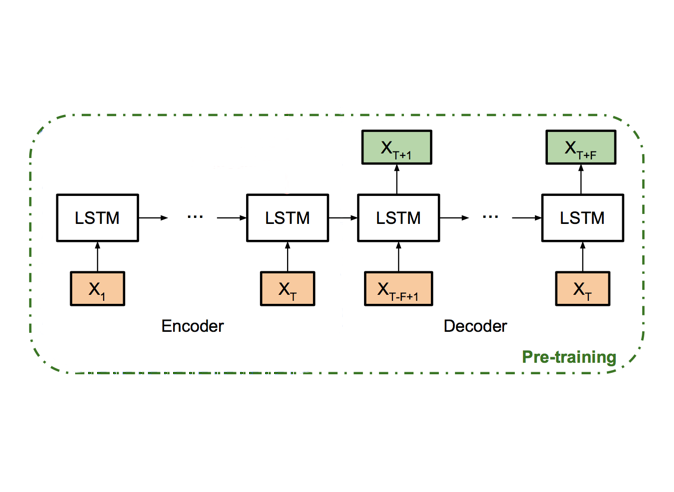
\includegraphics[width=0.9\columnwidth]{uber-train.png}
\caption{Modelo durante o Treinamento \citep{ubertime}}
\label{img:uber1}
\end{figure}


Durante o pré-treinamento a rede encoder-decoder consome sequências de $F + T$ dias
da série temporal. O encoder cria uma representação vetorial $h$ depois de
receber como entrada os primeiros $T$ dias da sequência. Então, $h$ é usado como
inicialização do estado interno do decoder, e esse então consume mais $F$
entradas da sequência. Para o decoder, se em uma iteração sua entrada é $X_i$,
então sua saída será comparada com $X_{i+1}$, e esse erro é propagado após lidas
todas as entradas para que a representação $h$ proveniente do encoder possa se
tornar mais informativa. \\


\begin{figure}[H]
  \centering
  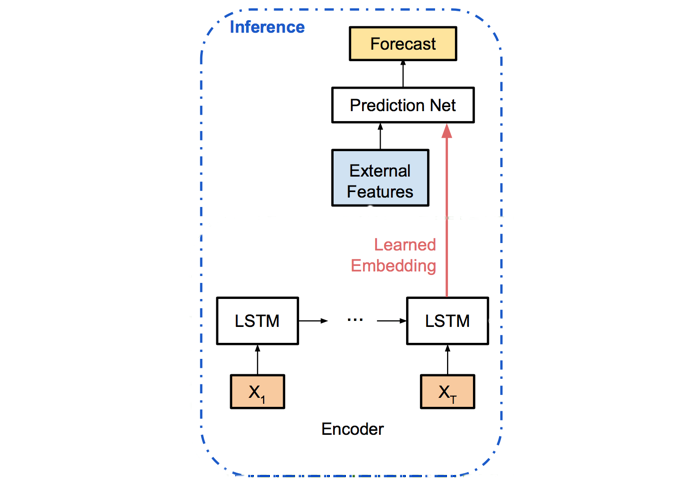
\includegraphics[width=0.9\columnwidth]{uber-predict.png}
  \caption{No módulo de inferência usamos uma rede neural simples para gerar
    predições a partir da codificação aprendida durante o pré-treino \citep{ubertime}}
  \label{img:uber2}
\end{figure}




Esse modelo também possui outra característica importante. Todas as camadas da
redes neurais que compõe o encoder, o decoder e o forecaster possuem
Dropout com probabilidade $p$. Ou seja, podemos usar a técnica do Monte
Carlo Dropout para estimar a variância de cada predição feita por esse modelo. A
rede então se torna um modelo bastante robusto para consumir séries temporais,
assim realizando predições e incertezas.\\


Essa capacidade do modelo o torna mais interessante do que meramente usar uma
rede LSTM para o problema de regressão. Agora iremos definir como a informação
de incerteza pode ser calculada usando esse modelo. \\

Para esse problema usamos a verossimilhança $p(y |f^\theta(x))$.
Onde $f^\theta(.)$ é a rede Encoder-Forecaster após o treino.
Como estamos lidando com regressão, podemos especificar ainda essa distribuição
como \citep{ubertime}:  

\begin{equation}
  \label{eq:reg}
 p(y| \theta,x) \sim \mathcal{N}(f^{\theta}(x),\,\sigma^2)
\end{equation}

Desejamos encontrar a distribuição $p(y^*| x^*)$ para dados inéditos. Seguindo
a formalização bayesiana, é necessário marginalizar os parâmetros do modelo da
verossimilhança, i.e. resolver a Integral~\ref{eq:int}. Para esse modelo, como
para muitos outros de interesse, essa integral é intratável. No trabalho
\citep{ubertime}, os autores estudam a variância de $p(y^{*} | x^{*})$ que
quantifica a incerteza das predições. Primeiro essa variância é decomposta pela
lei da variância total, e seus fatores são aproximados independentemente: 

\begin{equation}
   Var[y^* | x^*] = Var[\mathop{\mathbb{E}}(y^* | \theta,x^*)] + \mathop{\mathbb{E}}[Var(y^* | \theta,x^*)]
   \label{eq:vartot}
 \end{equation}

$\mathbb{E}[y^* | \theta,x^*]$ é a verossimilhança do modelo, ou seja:

\[
  Var[\mathbb{E}(y^* | \theta,x^*)] = Var[f^\theta(x^*)]
\]

$Var[f^\theta(x^*)]$ representa a incerteza do modelo, e a estimativa desse valor será feito pela técnica do MC Dropout. A variância
será aproximada pela variância amostral de $B$ predições estocásticas calculadas
na rede com camadas de Dropout ativadas. Seja $\{\hat{y}^*_{(1)}=f^{\theta_{(1)}}(x^*),\hat{y}^*_{(2)}=f^{\theta_{(2)}}(x^*), \dots
\hat{y}^*_{(B)}=f^{\theta_{(B)}}(x^*)\}$ o vetor de predições amostrado dessa forma, e $\bar{y}^*$ sua
média amostral, temos: \\

\[   Var[f^\theta(x^*)] \sim \eta_1^2 = \frac{1}{B}\sum^B_{B=1}(\hat{y}^*_{(B)} - \bar{y}^*)^2  \]

O termo $\mathop{\mathbb{E}}[Var(y^* | \theta,x^*)]$ da Equação~\ref{eq:vartot}, o
ruído inerente do modelo, será estimado com um conjunto de dados de validação.
Sejam $(X',Y')$ dados de validação, com
$V$ entradas. Esses dados são independentes do modelo
treinado $f^\theta(.)$, então podemos usá-los para estimar o ruído inerente do
modelo: \\

\[
  \mathop{\mathbb{E}}[Var(y^* | \theta,x^*)] \sim \eta_2^2 = \frac{1}{V}\sum^V_{V=1}(y'_v - f^\theta(x'_v))^2
\]



A Equação~\ref{eq:vartot} fica resumida em:


\[ Var[y^* | x^*] \sim \eta^2_1 + \eta^2_2 \] 

O desvio-padrão total do modelo é então calculado por:

\[
  \eta = \sqrt{\eta^2_1 + \eta^2_2}  
\]


\subsection{Modelo DeepAR}

O modelo \textit{DeepAR}, proposto em \citep{deepar}, é baseado em redes neurais
recorrentes auto-regressivas. Essa classe de modelos, que é bastante usada em
econometria, usa saídas passadas como entradas para o cálculo de próximos
valores. Dessa maneira em tese esses modelos podem gerar predições em horizontes
de tempo arbitrários no futuro.
Usa-se a função de verossimilhança binomial para que o modelo seja capaz
de realizar predições probabilísticas.

O modelo é descrito pela seguinte equação, onde $h$ é uma RNN implementada com células de LSTMs:

\[
h_{i,t} = h(h_{i,t-1},y^*_{i,t-1},x_{i,t}, \theta)
\]

O modelo é treinado em um conjunto de diversas séries temporais $y_i$ do
processo em estudo, todas representando o mesmo período de tempo. Nota-se que o estado da RNN tem como argumento o estado anterior e os parâmetros de entrada, mas também a saída da iteração passada do modelo, $y^*_{i,t-1}$. \\

A verossimilhança do modelo, $p(y_{i,t} | \mu,\sigma)$, é uma distribuição fixa
cujos parâmetros $\mu, \sigma$ são dados por uma função determinística da saída $h$ do modelo. Usaremos uma função de verossimilhança binomial já que estamos otimizando um objetivo de regressão, assim como na Equação~\ref{eq:logver1}:
\[
  p(y | \mu,\sigma) = {(2\pi\sigma^2)}^{-\frac{1}{2}} \exp(-  \frac{-y - \mu^2}{2\sigma^2})  
\]

A média $\mu$ e o desvio-padrão $\sigma$ são calculados diretamente pela saída do modelo. Para a média, usamos uma transformação linear parametrizada por $W_{\mu},b_{\mu}$. No caso do desvio-padrão, para garantirmos que ele seja maior que 0, usamos uma função \textit{softplus} após uma transformação linear análoga ao caso da média, parametrizada por  $W_{\sigma},b_{\sigma}$.\\

\begin{alignat}{3}
  \mu(h_{i,t}) &= W_{\mu}h_{i,t} + b_{\mu} \\ 
  \sigma(h_{i,t}) &= \log(1 + \exp(W_{\sigma}h_{i,t}+ b_{\sigma}))
\end{alignat}


\subsubsection{Treinamento}


O modelo possui uma etapa de treinamento e uma etapa de validação. O Diagrama~\ref{fig:deepartrain} ilustra como o modelo se comporta em cada um desses momentos: \\


\begin{figure}[H]
  \centering
  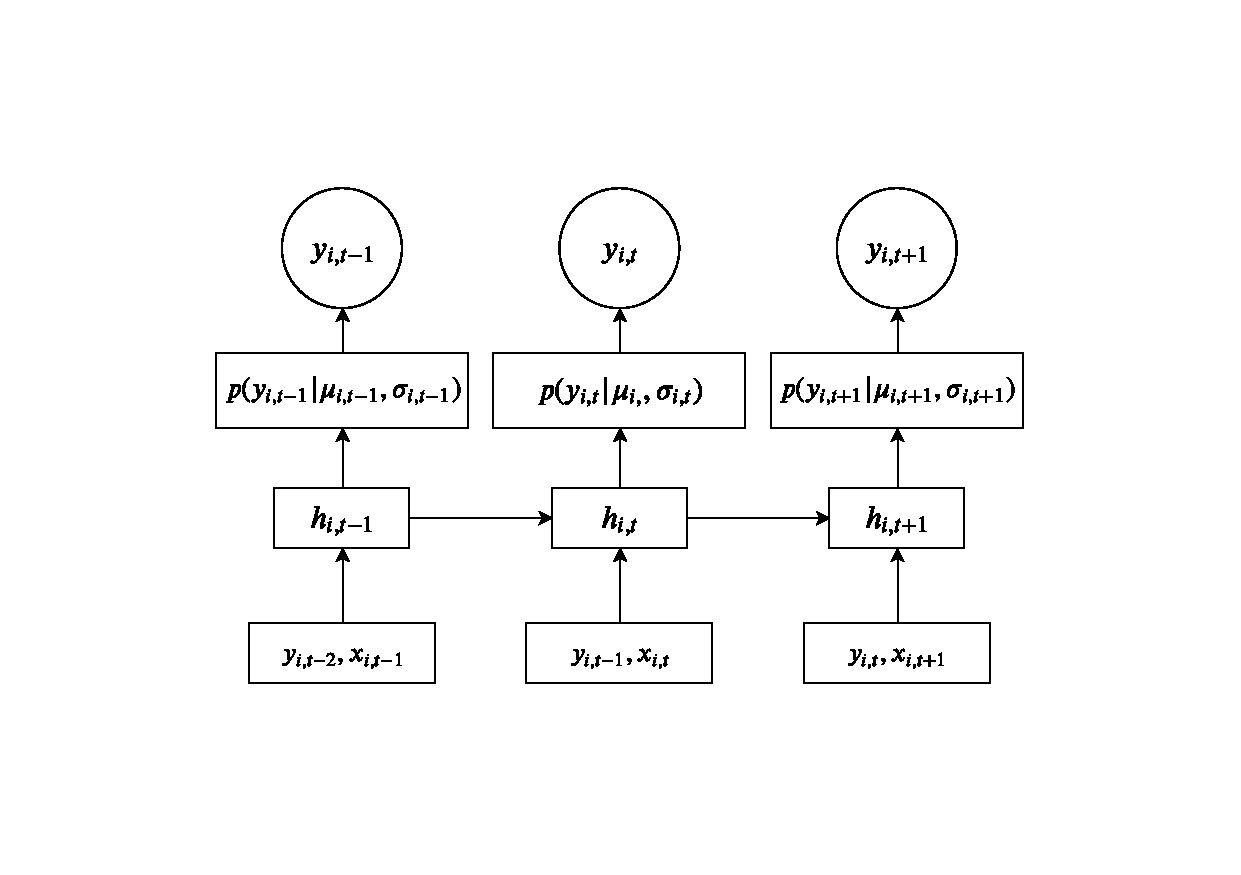
\includegraphics[width=0.9\columnwidth]{deepar-train.pdf}
  \caption{Para o treino, o modelo é guiado por anotações reais de valores
    passados da série alvo $y$ e as variáveis independentes $x$. Usamos o estado
  $h$ da rede LSTM a cada iteração temporal para calcular $\mu$  e $\sigma$.
  Esses valores são então usados no calculo da verossimilhança $p(y |
  \mu,\sigma)$, o valor que é minimizado.}
  \label{fig:deepartrain}
\end{figure}

%% lembrar que p(y | \mu,\sigma) == l(z| \theta) no diagrama!
%%

O treinamento do modelo é feito pela maximização da log-verossimilhança: \\

\begin{equation}
  \mathcal{L} = \sum^n_{t=1}{\log p(y_{i,t} | \mu_{i,t},\sigma_{i,t})}
  \end{equation}

Durante a etapa de predição, os valores calculados de $\mu$ e $\sigma$ são
usados como parâmetros de uma distribuição normal que caracteriza a distribuição
de cada predição $y^*$.


\begin{figure}[H]
  \centering
  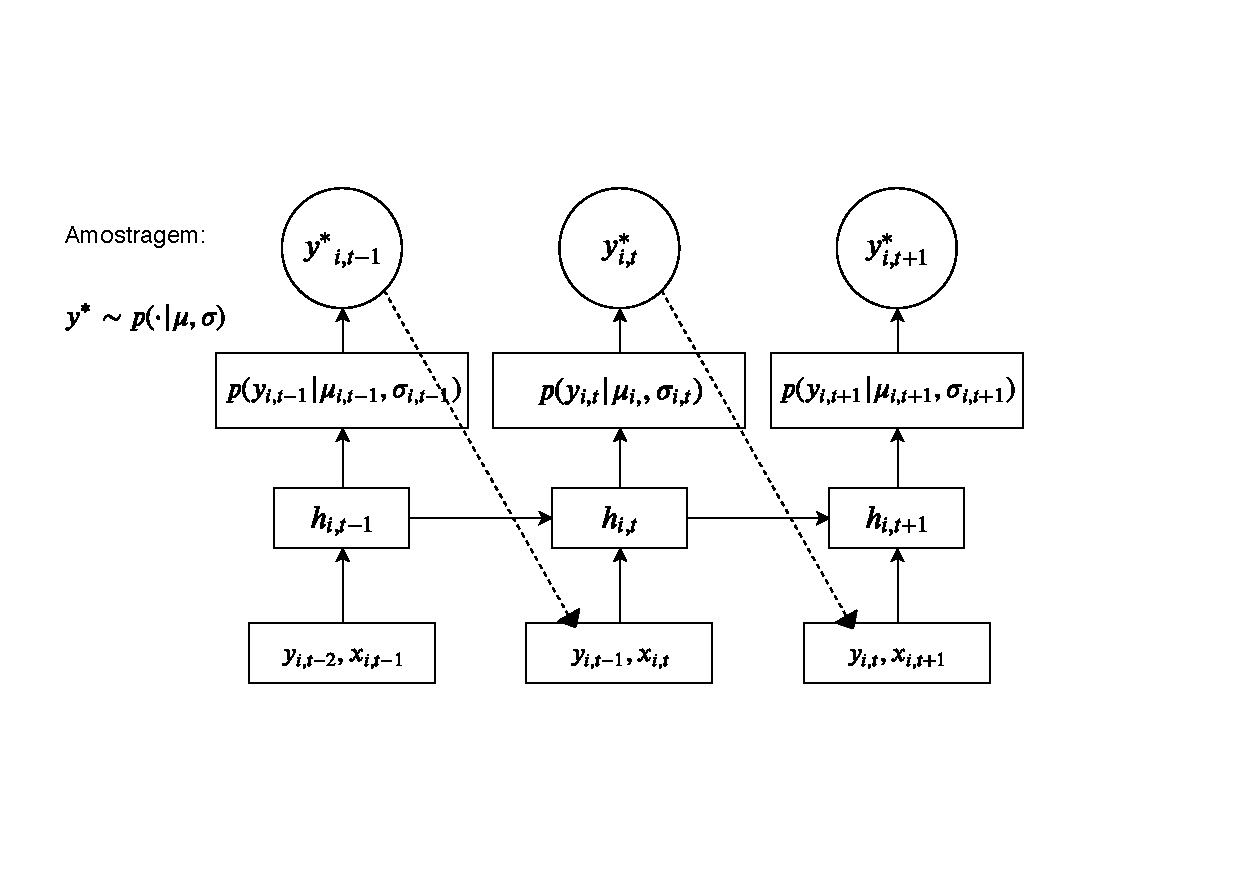
\includegraphics[width=0.9\columnwidth]{deepar-pred.pdf}
  \caption{Se desejarmos prever mais de um valor da série-alvo $y$ no futuro. O
    modelo é realimentado com os valores amostrados de $y^*$ e a rede continua a
  realizar predições.}
  \label{fig:deepartrain}
\end{figure}


Uma saída $y^*_{i,t}$ do modelo é calculada por meio de uma amostragem da Gaussiana determinada pela média e variância calculadas: \\

\[
 y^*_{i,t} \sim \mathcal{N}(\mu_{i,t},\sigma_{i,t}) 
\]

\subsection{Modelo com Deep Factors}

O modelo \textit{Deep Factors with Gaussian Process} \citep{deepfactors} separa o problema de predição em uma parte \textbf{local}, modelada por um Processo Gaussiano que gera incertezas, e uma parte \textbf{fixa}, modelada por uma rede neural recorrente treinada em diversas séries temporais do mesmo domínio.


Um Processo Gaussiano é uma coleção de variáveis aleatórias,
sendo que qualquer subconjunto finito das mesmas é distribuído normalmente \citep{gpml}. \\

Um Processo Gaussiano é descrito completamente pela sua função de média e sua função de covariância. Usamos essas duas funções para amostrar o processo estocástico $f(x)$ que está sendo modelado: \\

\[
f(x) \sim \mathcal{GP}( m(x), K(x,x'))
\]

É comum que se escolha como função média apenas a constante 0 \citep{gpml}.  A função de covariância, as vezes chamada de Kernel, deve especificar a covariância entre os pares de variáveis aleatórias (i.e. os dados), para problemas de regressão é usual escolhermos um Kernel que relacione uma medida de distância das variáveis de entrada. Como por exemplo o \textit{quadrado da função exponencial}: \\

\[
  K(x,x') = \exp(-\frac{1}{2}\abs{x - x'}^2)
\]


\subsubsection{Modelo Generativo}

O modelo Deep Factors então é composto por duas partes, a combinação linear de ambas é a saída do modelo i.e. a emissão de valores de saída amostrados: \\

\[
  \textbf{Gerador da parte fixa aprendida globalmente: }  f_{i,t} = W_ig_t(x_{i,t})
\]

A função $g_t$ é uma RNN, no caso desse trabalho uma célula LSTM, que recebe como entrada um certo número $T$ de passos da série temporal, e então emite como saída um horizonte finito $F$ de predições.


\[
  \textbf{Gerador de ruído local: }  r_i \sim \mathcal{GP} (0, K_i(.,.))
\]
O ruído é gerado por um Processo Gaussiano com média 0 e função de covariância
exponencial. O Processo gera incertezas a partir da matriz de covariância
calculada com todas as predições da parte global do modelo. Seja $f_i$ um vetor
de predições com $T$ entradas calculado pela rede LSTM para a série temporal $i$, a matriz de covariância
terá a forma:  

\[
  \begin{bmatrix}
    1& K(f_{i,1},f_{i,2}) & \dots &K(f_{i,1},f_{i,T}) \\ 
    K(f_{i,2},f_{i,1}) &1  & \dots & K(f_{i,2},f_{i,T})\\ 
    \vdots &  \vdots  & \ddots & \vdots\\
    K(f_{i,T},f_{i,1})& K(f_{i,T},f_{i,2}) & \dots & 1 
  \end{bmatrix} 
\]

\[
  \textbf{Emissão: }  y^*_{i,t} \sim p(. | u_{i,t}) , u_{i,t} = r_{i,t} + f_{i,t}  
\]
A emissão ira combinar efeitos globais e ruído local para gerar as predições
finais amostrando-se a variável latente $u$:
  

\subsubsection{Treinamento}

Para o problema de regressão, podemos assumir que $p(. | u_{i,t})$ é distribuida
normalmente, então não precisamos de inferência para calcular a verossimilhança do modelo, que é dada por: \\

\[
p(y_{i}) = \mathcal{N}(f_i,K_i + \sigma_i^2\mathcal{I})
\]

O objetivo de treinamento é achar o conjunto de parâmetros da RNN e do Processo Gaussiano que maximizem a log-verossimilhança dos dados: \\
\[
\mathcal{L} = \sum_{t=0}^N{\log p(y_t|x_t)}
\]


%%% Local Variables:
%%% mode: latex
%%% TeX-master: "../quali"
%%% TeX-command-default: "latexmk"
%%% bibtex-file-path: "../bibliografia"
%%% End:
